\documentclass{beamer}
\DeclareFontShape{OT1}{cmss}{b}{n}{<->ssub * cmss/bx/n}{} 
\usetheme{Szeged}
\usecolortheme{beaver}
\usepackage{amsmath}
\usepackage{amsfonts}
\usepackage{mathbbol}
\usepackage{xcolor} % before tikz or tkz-euclide if necessary
\usepackage{tikz}
%\usepackage{tkz-euclide} % no need to load TikZ
%\usepackage{tikz-cd}
\usepackage{multirow}
\usepackage{lmodern}
\usepackage{bm}
\usepackage{subcaption}
%\usepackage{subfigure}


\usepackage[
backend=biber,
style=authoryear-icomp,
sortlocale=de_DE,
natbib=true,
url=false, 
doi=true,
eprint=false
]{biblatex}
\addbibresource{../Bibliography/main_ML.bib}
\usetikzlibrary{cd}


\titlegraphic{
\includegraphics[width=2cm]{../Figures/UAMS_RGB.png}
}


\title{CMDR Journal Club\\ Math Modeling for Bone-Cell Dynamics}
\author{Horacio G\'omez-Acevedo\\ Department of Biomedical Informatics\\
	University of Arkansas for Medical Sciences}

\begin{document}
	\begin{frame}[plain]
		\maketitle
	\end{frame}

\begin{frame}{Overview}
	\tableofcontents
\end{frame}

\section{Math Modeling}
\begin{frame}{}
	\begin{quote}
	Mathematicians are a kind of Frenchman. They translate into their own language whatever is said to them and forthwith the thing is utterly changed.\\
	Johann Wolfgang von Goeth
	\end{quote}
\end{frame}



\begin{frame}{Why Math Modeling?}

\begin{itemize}
	\item It is an attempt to introduce theoretical foundations to biological processes.
	\item It can also explain also some of the paradoxical observations.
	\item Based on "mechanistic" assumptions, models can produce useful predictions. 
	\item Once a model is "calibrated", it can accommodate extensions based on new biological findings. 
\end{itemize}	


\end{frame}
\subsection{Basic Ideas}
\begin{frame}{Compartmental Models}
The so-called \textbf{Compartmental Models} try to describe the dynamics of cell interactions among two or more well-characterized cell types.
 Some basic implicit assumptions about cell populations
\begin{itemize}
	\item The evolution of the population is described by rates (i.e., instant changes in population numbers).
	\item Cells are indistinguishable among the same type ($A$ and $B$ below). 
	\item $A$ and $B$ represent abundance of the given type. 
\end{itemize}
\end{frame}
\begin{frame}{Compartmental Models (cont)}
	
\begin{itemize}
\item Cells are entering (some progenitor cell) into the $A$ compartment at a certain rate $\pi_A$.
\item Cells leave the compartment (cell death) at the rate $\mu_A$ and $\mu_B$, respectively.
\item Cells evolve from Type $A$ into Type $B$ at a rate proportional to their abundance at a constant rate $\beta$.
\end{itemize}	

	\begin{figure}[h]
	\centering
	%	\begin{subfigure}{0.4\textwidth}
		%		\centering
		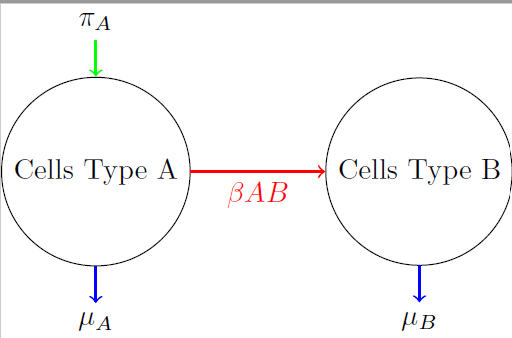
\includegraphics[scale=0.4]{../Figures/fig_compartment.png}
		%	\end{subfigure}
\end{figure}
	
\end{frame}

\begin{frame}{Compartmental Model Math}
The translation of this interaction is translated in the following system of (ordinary) differential equations

\begin{equation}
	\begin{split}
		A'&= \pi_A - \beta A B - \mu_A A \\
		B'&= \beta A B - \mu_B B
	\end{split}
\end{equation}
	\begin{figure}[h]
	\centering
	%	\begin{subfigure}{0.4\textwidth}
		%		\centering
		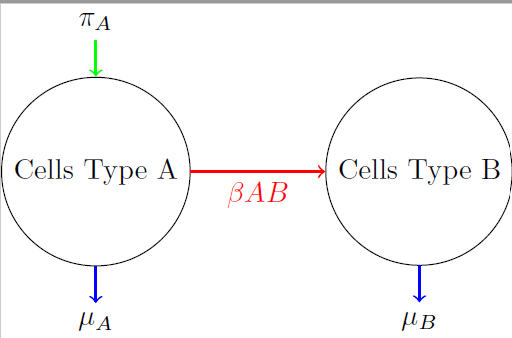
\includegraphics[scale=0.4]{../Figures/fig_compartment.png}
		%	\end{subfigure}
\end{figure}

\end{frame}

\begin{frame}{"Solving" the equations}
	For the above system, we can calculate the "steady state(s)". This means the point(s) that the trajectories will end up reaching (after potentially some very long time) or they are getting away from.
\begin{figure}[h]
	\centering
	%	\begin{subfigure}{0.4\textwidth}
		%		\centering
		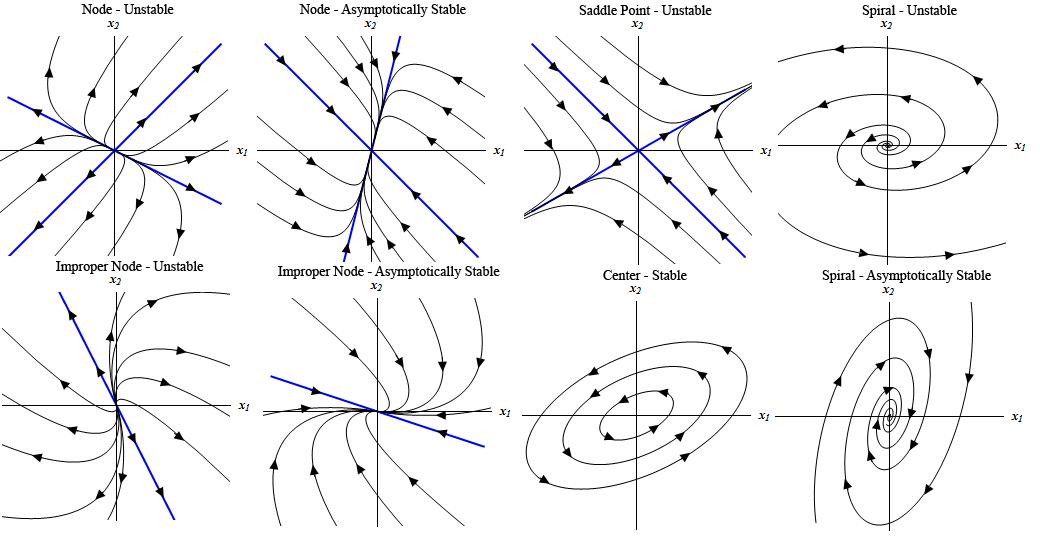
\includegraphics[scale=0.2]{../Figures/fig_dyn_sys.jpg}
		\caption{\href{https://discourse.julialang.org/t/plotting-dynamical-systems-trajectories/46166}{dynamical systems}}
		%	\end{subfigure}
\end{figure}	
	
\end{frame}

\begin{frame}{"Solving" the equations (cont)}
	In general, it is relatively hard to calculate those steady states and determine (locally) their behavior (attractor  or repelor) (\textcolor{red}{Mathematical issue})
	
	Instead, we solve the equations "numerically". Meaning, we write code to simulated the trajectories (e.g., Matlab) for a given set of parameters ($\pi_A$, $\beta$, etc.)
\begin{figure}[h]
	\centering
	%	\begin{subfigure}{0.4\textwidth}
		%		\centering
		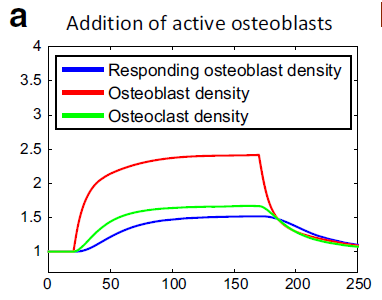
\includegraphics[scale=0.45]{../Figures/fig_numeric_sol.png}
	
		%	\end{subfigure}
\end{figure}		 
	
	
\end{frame}

\begin{frame}{In Silico Simulations}
A great deal of time is spent calculating the parameters from a given established system
\begin{itemize}
	\item Using other literature sources
	\item Making simulations based on newly produced data	
\end{itemize}

The ultimate goal is to produce a tuned \textit{in silico} system based on  equations that mimic fundamental biological concepts. Then, we can explore scenarios and test biological hypothesis. 



\end{frame}


\section{Paper}
\begin{frame}{Today's paper}
	\begin{figure}[h]
		\centering
		%	\begin{subfigure}{0.4\textwidth}
			%		\centering
			
\includegraphics[scale=0.4]{../Figures/lemaire_paper_2019.png}
			%	\end{subfigure}
	\end{figure}
\end{frame}

\subsection{Main Model}
\begin{frame}{Picture First}
		\begin{figure}[h]
		\centering
		%	\begin{subfigure}{0.4\textwidth}
			%		\centering
			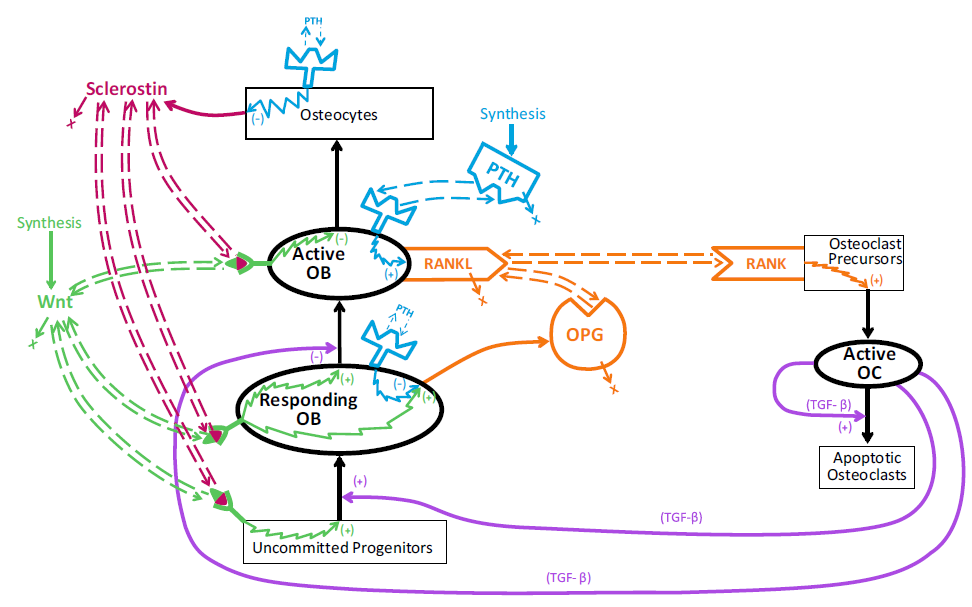
\includegraphics[scale=0.5]{../Figures/fig_lemaire_fig1.png}
			%	\end{subfigure}
	\end{figure}
\end{frame}

\begin{frame}{Cell Compartment Equations}

\begin{equation}
	\begin{split}
	R' &= D_R \pi_C \pi_W - D_B \frac{\pi_W}{\pi_C} R\\
	B' &= D_B \frac{\pi_W}{\pi_C} R - \frac{k_e^B}{\pi_W}B\\
	C' &= D_C \pi_L - k_e^C \pi_C C 
	\end{split}
\end{equation}
According to the model $D_R$, $D_B$ and $D_C$ are constant differentiation rates, $k_e^B$, and $k_e^C$ are constant elimination rates. 

\end{frame}

\subsection{Ligands Competition}
\begin{frame}{Ligands Models}
	The modeling follows the enzymatic theory of Michaelis-Menten.
	In brief, if we have a substrate $S$ reacting with an enzyme $E$ to form a complex $SE$ can be modeled as
\begin{center}
\begin{tikzcd}[ampersand replacement=\&, column sep=small]
	S +E  \arrow[r,shift left, "k_1"] \& S\circ E \arrow[l,shift left,"k_{-1}"]  
\end{tikzcd}
\end{center}	

\begin{equation}
\frac{d S \circ E}{dt}= k_1 S \cdot E - k_{-1} S \circ E
\end{equation}

When the text refers that equations are considered at "steady state" it means that 
\begin{equation*}
	k_1 S \cdot E = k_{-1} S \circ E
\end{equation*}
	
\end{frame}

\begin{frame}{Ligand Models (cont)}
			\begin{figure}[h]
		\centering
		%	\begin{subfigure}{0.4\textwidth}
			%		\centering
			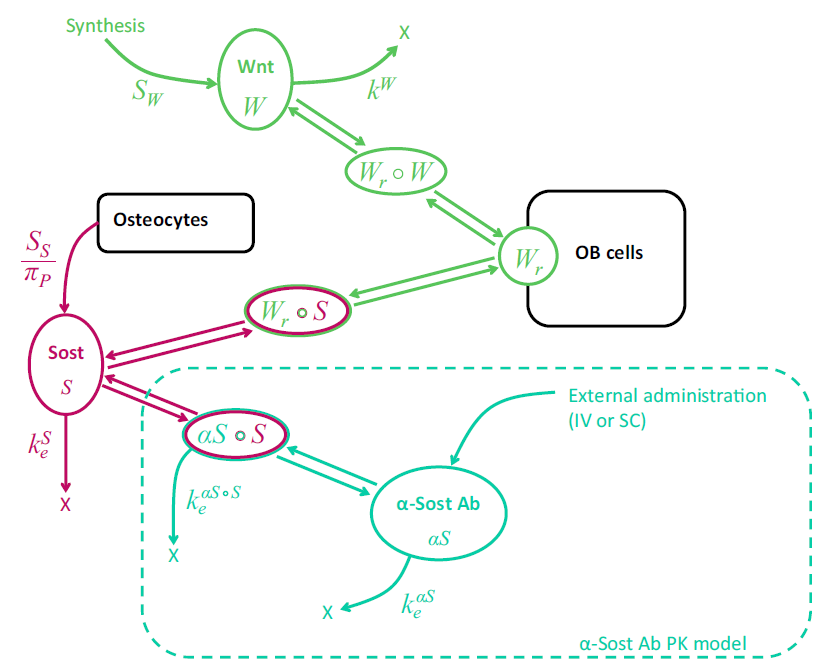
\includegraphics[scale=0.45]{../Figures/fig_lemaire_fig2.png}
			%	\end{subfigure}
	\end{figure}
	
\end{frame}

\begin{frame}{Binding to LPR5/6}
The attachment of Wnt to the receptor $W_r$ is taken at the steady state. 
The equations for binding of Wnt receptor and sclerostin are

\begin{equation}
	\begin{split}
		\frac{d W_r \circ S}{dt} &= k_9 S \cdot W_r - k_{10} W_r \circ S \\
		\frac{d \alpha S  \circ S}{dt} &= k_{13} S \cdot \alpha S - k_{14} \alpha S \circ S -k_e^{\alpha S \circ S} \alpha S \circ S 
	\end{split}
\end{equation}
The second equation represents the presence of an antibody for Sost
\end{frame}

\subsection{Parameters}
\begin{frame}{Parameter Estimation}
\begin{figure}[h]
	\centering
	%	\begin{subfigure}{0.4\textwidth}
		%		\centering
		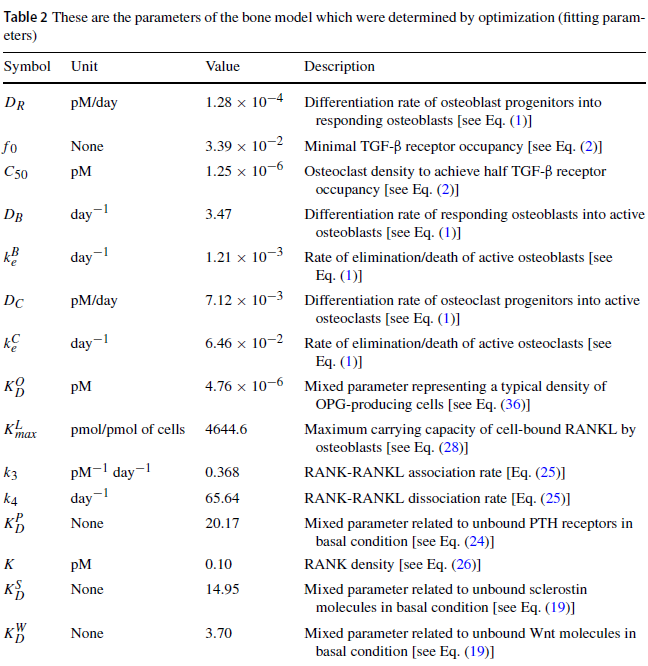
\includegraphics[scale=0.45]{../Figures/fig_lemaire_table2.png}
		%	\end{subfigure}
\end{figure}	
\end{frame}

\begin{frame}{"Optimization"}
This part is not the traditional (formal) optimization process. 

The authors try to place some reasonable constrains (i.e. the dynamics reaches steady stead in less than 500 days)

The scenarios ("objectives") are mostly a sanity check for the model. The notation $R\nearrow $ represent a "significant" increase in the steady-state value of the mentioned species should be observed after perturbations (e.g., drug) is applied.
\end{frame}

\begin{frame}{"Optimization" (cont)}
	\begin{figure}[h]
		\centering
		%	\begin{subfigure}{0.4\textwidth}
			%		\centering
			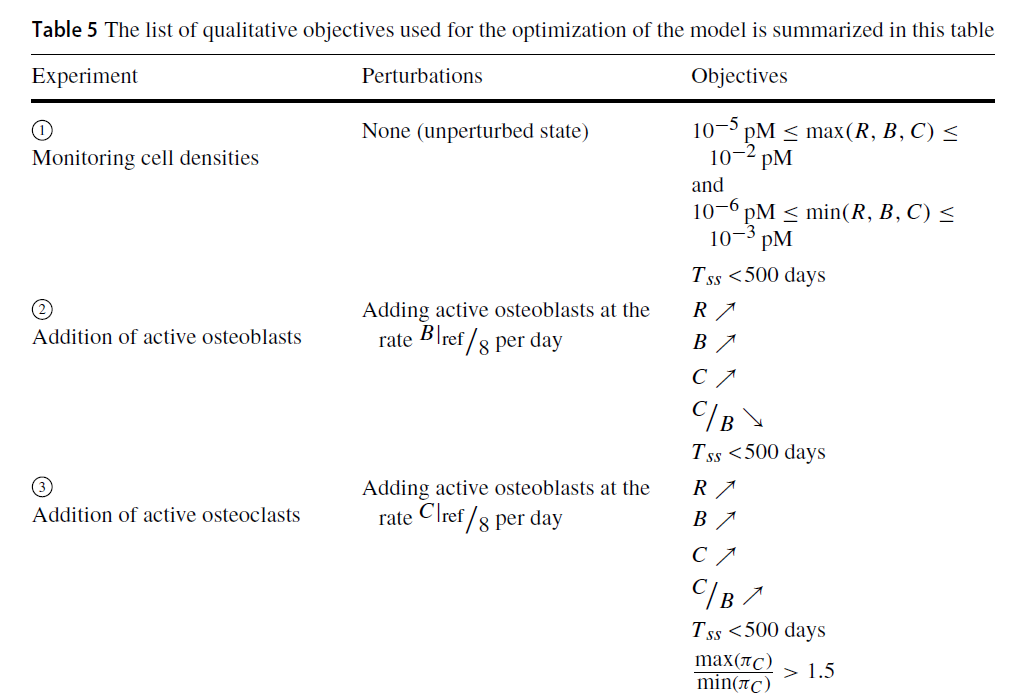
\includegraphics[scale=0.45]{../Figures/fig_lemaire_table5.png}
			%	\end{subfigure}
	\end{figure}	
\end{frame}

\begin{frame}{Adding PK}
	A two-compartment model for hPTH was used
	\begin{figure}[h]
	\centering
	%	\begin{subfigure}{0.4\textwidth}
		%		\centering
		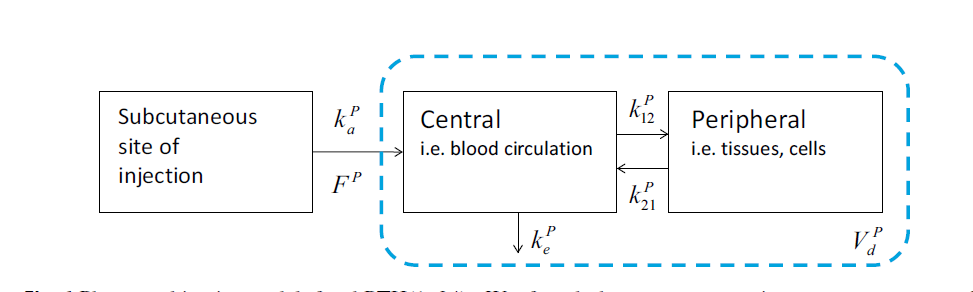
\includegraphics[scale=0.45]{../Figures/fig_lemaire_fig6.png}
		%	\end{subfigure}
\end{figure}		
	
\end{frame}
\begin{frame}{PK model for Anti-RANKL}
	\begin{figure}[h]
	\centering
	\begin{subfigure}{0.4\textwidth}
		%		\centering
		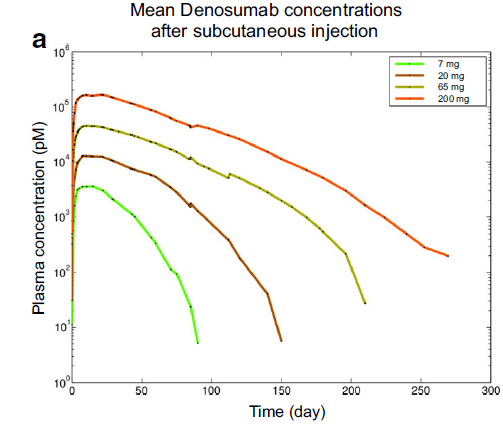
\includegraphics[scale=0.45]{../Figures/fig_lemaire_fig9a.png}
	\end{subfigure}
	\begin{subfigure}{0.4\textwidth}
	%		\centering
	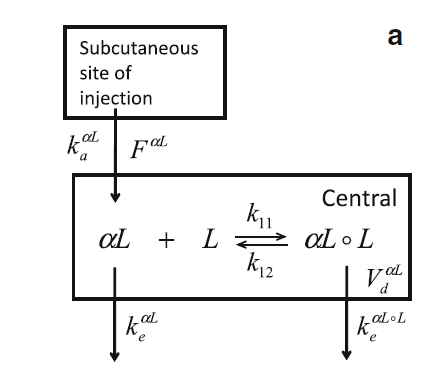
\includegraphics[scale=0.45]{../Figures/fig_lemaire_fig10a.png}
	\end{subfigure}
\end{figure}
	

\end{frame}
\begin{frame}{PK model for Anti-RANKL}
They used a one compartment model described by the equation
\begin{equation}
	\begin{split}
	\frac{d\alpha L}{dt}&= P^{\alpha L}(t)- k_e^{\alpha L} \cdot \alpha L - k_e^{\alpha L \circ L} \cdot \alpha L \circ L\\
	&=P^{\alpha L}(t)- \left( 
	k_e^{\alpha L}  + \frac{k_e^{\alpha L \circ L}}{K_d^{\alpha L}} L  \right) \alpha L 
	\end{split}
\end{equation}

\end{frame}

\section{Model Simulations}


\begin{frame}{Denosumab single dose simulation}
\begin{figure}[h]
		\centering
		%	\begin{subfigure}{0.4\textwidth}
			%		\centering
			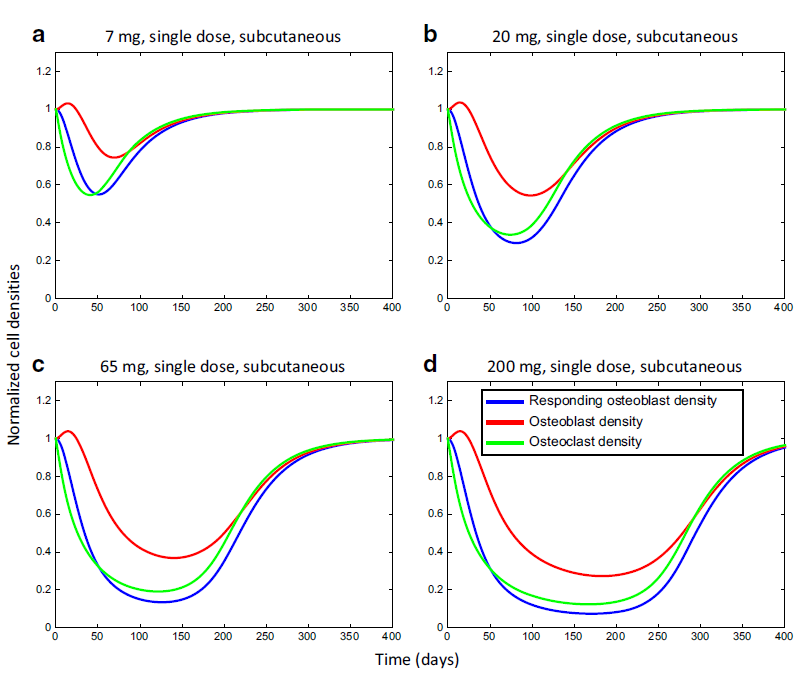
\includegraphics[scale=0.45]{../Figures/fig_lemaire_fig14.png}
			%	\end{subfigure}
	\end{figure}	
\end{frame}	

\begin{frame}{Combination of Therapies (in sillico)}
\begin{figure}[h]
	\centering
	%	\begin{subfigure}{0.4\textwidth}
		%		\centering
		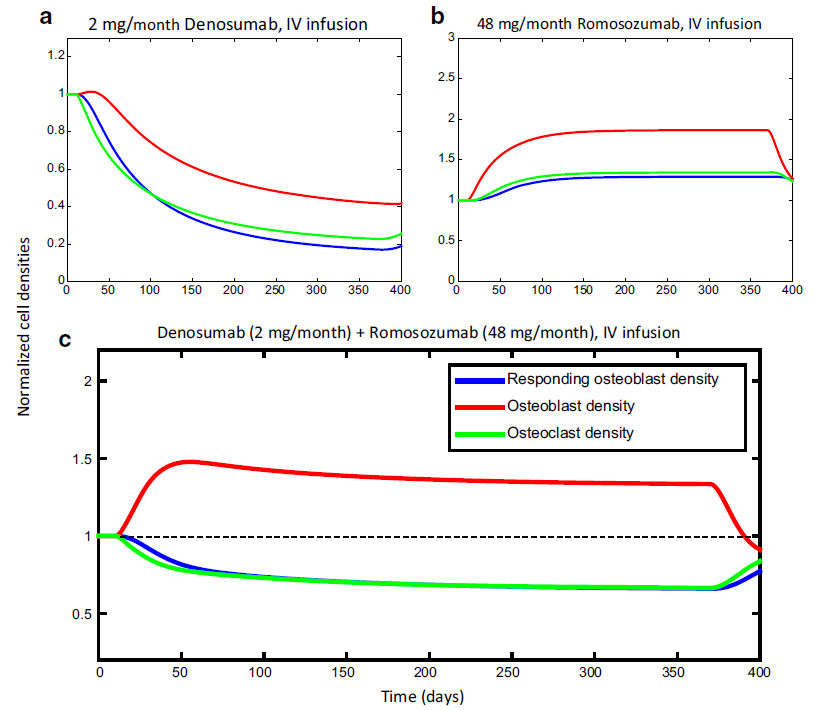
\includegraphics[scale=0.45]{../Figures/fig_lemaire_fig16.png}
		%	\end{subfigure}
\end{figure}	

	
\end{frame}

\begin{frame}{Multiple injections}
\begin{figure}[h]
	\centering
	%	\begin{subfigure}{0.4\textwidth}
		%		\centering
		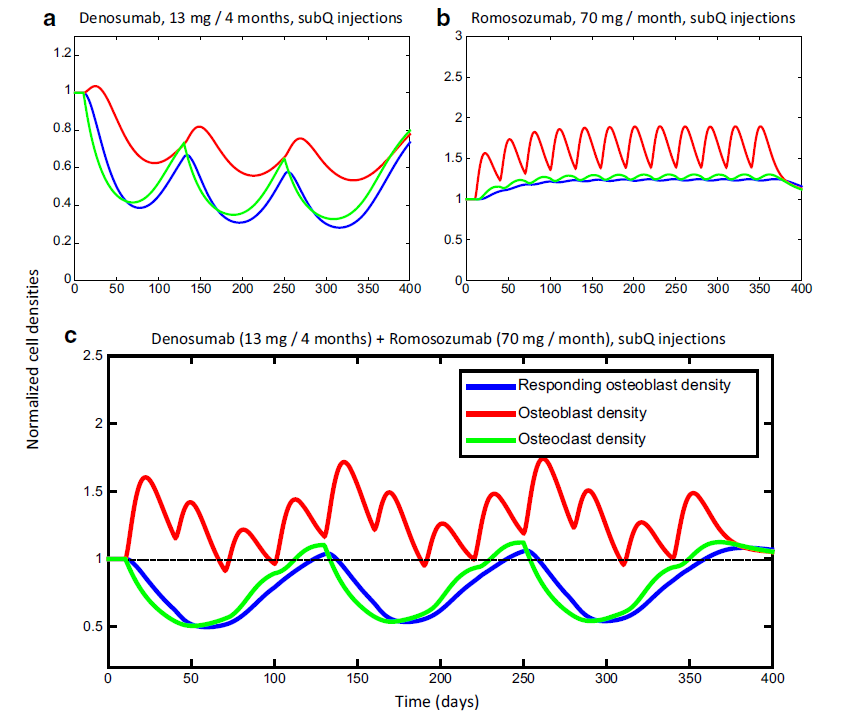
\includegraphics[scale=0.45]{../Figures/fig_lemaire_fig17.png}
		%	\end{subfigure}
\end{figure}	
\end{frame}

\begin{frame}{Dosing Regimens}
\begin{figure}[h]
	\centering
	%	\begin{subfigure}{0.4\textwidth}
		%		\centering
		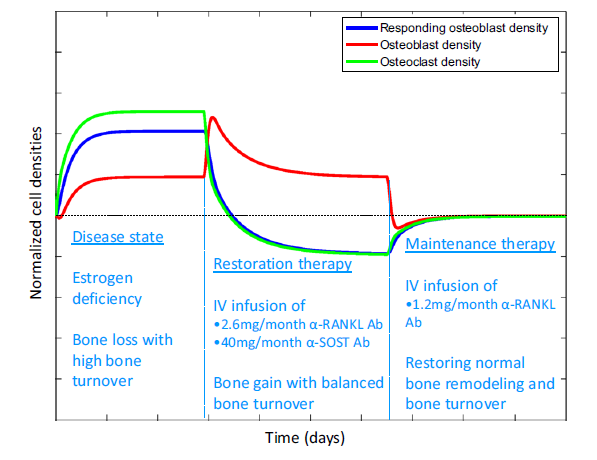
\includegraphics[scale=0.45]{../Figures/fig_lemaire_fig18.png}
		%	\end{subfigure}
	\caption{Combination therapy for postmenopausal osteoporosis}
\end{figure}		
\end{frame}

\section{Conclusions}

\begin{frame}{Math Models}
	\begin{itemize}
		\item Several groups around the globe are incorporating math modeling. Notably, Peter Pivonka (Queensland).
		\item Most of the publications have referenced the work from this group!
		\item There are many extensions to the basic model. 
	\end{itemize}
\end{frame}

\begin{frame}{Papers}
	\begin{figure}[h]
		\centering
		%	\begin{subfigure}{0.4\textwidth}
			%		\centering
			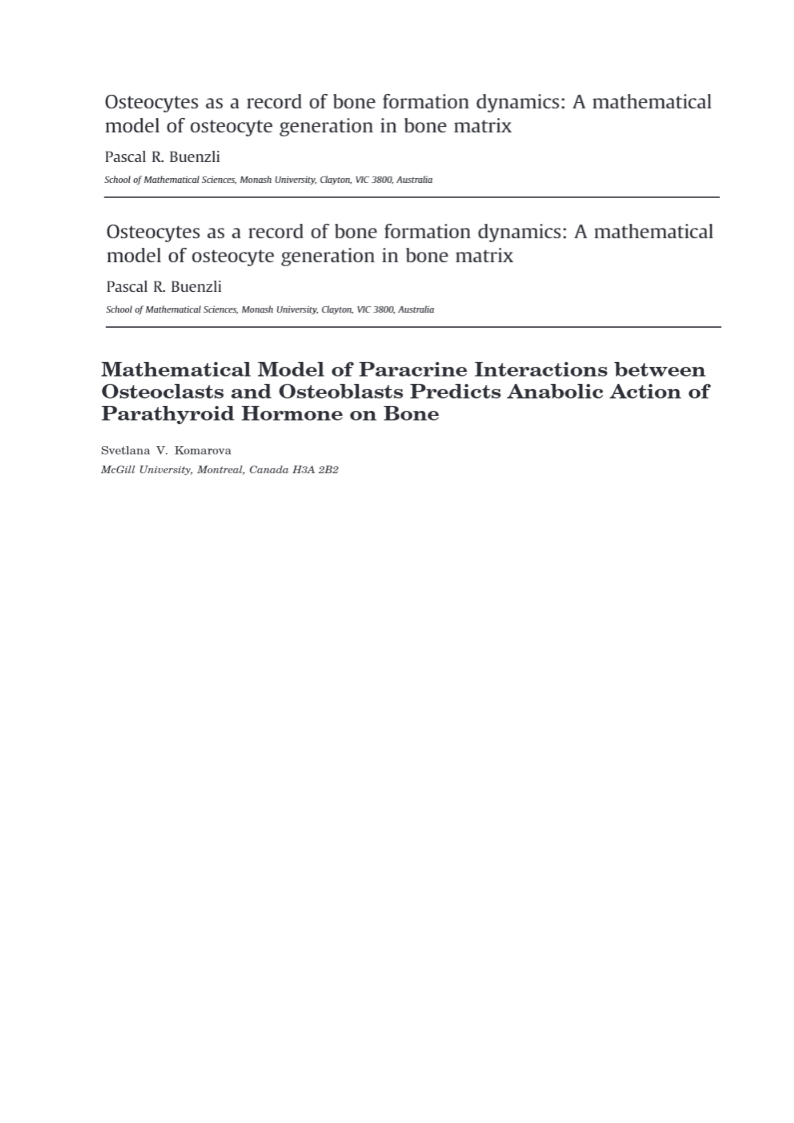
\includegraphics[scale=0.5]{../Figures/fig_papers_combined1-3.png}
			%	\end{subfigure}
	\end{figure}
\end{frame}

\begin{frame}{More Papers}
	\begin{figure}[h]
		\centering
		%	\begin{subfigure}{0.4\textwidth}
			%		\centering
			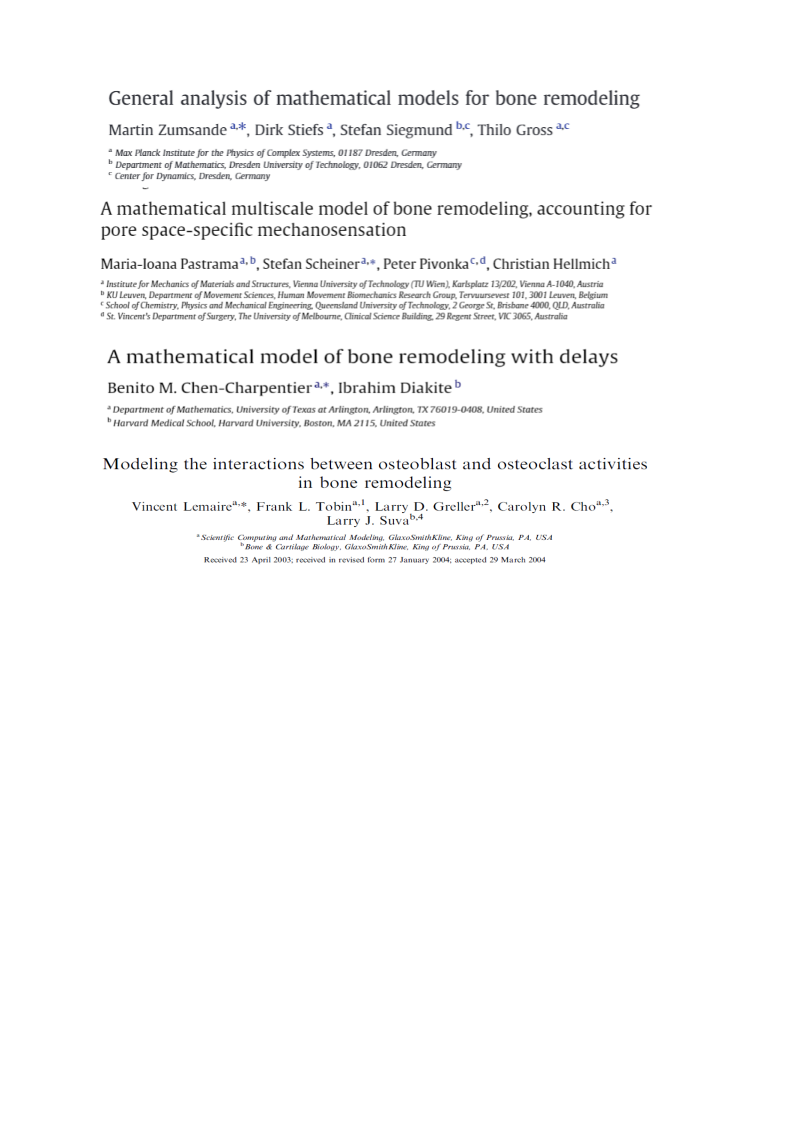
\includegraphics[scale=0.45]{../Figures/fig_papers_combined4-7.png}
			%	\end{subfigure}
	\end{figure}
\end{frame}


\begin{frame}{}
	\begin{quote}
		If the Lord Almighty had consulted me before embarking on creation I should have recommended something simpler\\
		Alphonso X (Alphonso the Wise) 1221-1284\\
		King of Castile and Leon
	\end{quote}
	
\end{frame}	



%\begin{frame}{References}
%	Materials and some of the pictures are from \citep{calin}.
%	\printbibliography 	
	
%	I have used some of the graphs by hacking TiKz code from StakExchange, Inkscape for more aesthetic plots and other old tricks of \TeX
	
%\end{frame}


\end{document}
